\documentclass{article}

\usepackage{amsmath,amssymb}
\usepackage{fullpage}
\usepackage{enumerate}
\usepackage{hyperref}
\usepackage{graphicx}
\usepackage{siunitx}
\graphicspath{{../logos/}}


\begin{document}

\setlength{\tabcolsep}{6pt}
\begin{center} \begin{tabular}{cccc}
	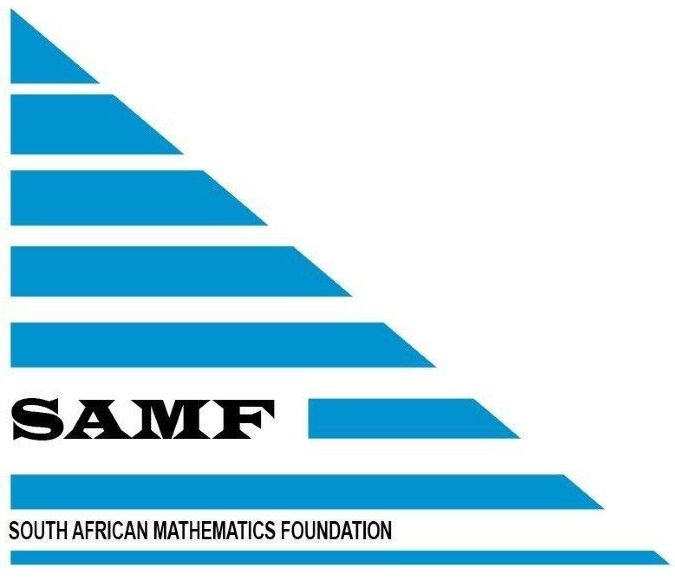
\includegraphics[height=56pt]{SAMF_logo.jpg} &
	
\includegraphics[height=56pt]{SAICA_logo.jpg} &
	
\includegraphics[height=56pt]{OM_Logo_Stacked_Vignette_on_White_RGB.jpg} &
	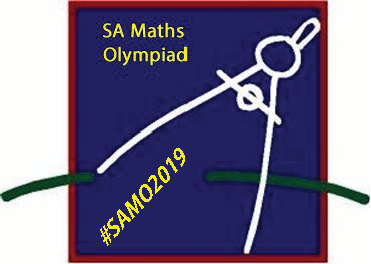
\includegraphics[height=56pt]{SAMO2019.png}
\end{tabular} \end{center}


\bigskip


\begin{center}
	\textbf{\Large Senior Monthly Problem Set Solutions for when it would have been IMO Season :(}
\end{center}

\begin{enumerate}

\medskip
\item[1.] % Silk Road Maths Competition, 2012
\textit{Let $ABCD$ be a cyclic quadrilateral with $AD \parallel BC$. Let $X$ be the midpoint of arc $AD$ that does not contain point $C$ and $P$ be a point on the tangent to the circle at $C$ such that $\angle CPX = 90 \si{\degree} $. Prove that $BC = 2 CP$.}

If $O$ is the circumcenter of $ABCD$, then line $OX$ intersects $BC$ at it's midpoint $M$. and $\angle XMC = 90 \si{\degree}$. The desired result is thus equivalent to $CM = CP$. In triangle $CMX$ and triangle $CPX$, we have that line $CX$ is common and $\angle CMX = 90 \si{\degree} = \angle CPX$. Thus, the triangles will be congruent, and the desired result proven, if $\angle MCX = \angle PCX$. Notice that $\angle PCX = \angle CBX$ by the tan-chord theorem. Since $\triangle XBM \equiv \triangle XCM$, we have that $\angle MCX = \angle MBX = \angle CBX = \angle PCX$, and we are done.


\medskip
\item[2.] % AoPS, 2020
\textit{For $n,m\in\mathbb{N}$ let $S_{n,m}$ be the set of all increasing integer sequences $x_{1},x_{2},\ldots,x_{nm}$, where $0\leq x_i\leq nm$ and satisfying $n \mid x_{1} + x_{2} + \cdots +x_{nm}$. Prove that exactly half of the elements of $S_{n,m}$ have $x_{nm}=nm$.}



\medskip
\item[3.] % IMC 2015, Day 1, Problem 2, Stephan Wagner
\textit{Let $B: \mathbb{N} \rightarrow \mathbb{N}$ be a function such that $B(n)$ is the number obtained by changing every $0$ in the binary expansion of $n$ to a $1$ and every $1$ to a $0$. Leading $0$'s are ignored in the binary expansion of $n$. Prove that for any positive integer $k$}

$$\sum_{r=1}^{k} B(r) \le \frac{k^2}{4}$$

\textit{When does equality occur?}

If $r$ and $k$ are positive integers with $2^{r - 1} \le k < 2^r$ then $k$ has $r$ binary digits, so $k + B(k) = 2^r - 1$.

Assume that $2^{s - 1} - 1 \le n \le 2^s - 1$, then:
\begin{align*}
\frac{n(n + 1)}{2} + \sum_{k = 1}^{n} B(k) &= \sum_{k = 1}^{n} (k + B(k)) \\
&= \sum_{r = 1}^{s - 1} \sum_{2^{r - 1} \le k < 2^r} (k + B(k)) + \sum_{2^{s - 1} \le k \le n} (k + B(k)) \\
&= \sum_{r = 1}^{s - 1} 2^{r - 1} \cdot (2^r - 1) + (n - s^{s - 1} + 1) \cdot (2^s - 1) \\
&= \sum_{r = 1}^{s - 1} 2^{2r - 1} - \sum_{r = 1}{s - 1} 2^{r - 1} + (n - 2^{s - 1} + 1)(2^s - 1) \\
&= \frac{2}{3} (4^{s - 1} - 1) - (2^{s - 1} - 1) + (2^s - 1)n - s^{2s - 1} + 3 \cdot 2^{s - 1} - 1 \\
&= (2^s - 1)n - \frac{1}{3} 4^s + 2^s - \frac{2}{3}
\end{align*}

and therefore

\begin{align*}
	\frac{n^2}{4} - \sum_{k = 1}^{n} B(k) &= \frac{n^2}{4} - ((2^s - 1)n - \frac{1}{3}4^s + 2^s - \frac{2}{3} - \frac{n(n + 1)}{2}) \\
	&= \frac{3}{4}n^2 - (2^s - \frac{3}{2})n + \frac{1}{3}4^s - 2^s + \frac{2}{3} \\
	&= \frac{3}{4}(n - \frac{2^{s + 1} - 2}{3})(n - \frac{2^{s + 1} - 4}{3})
\end{align*}

Notice that the difference of the last two factors is less than $1$, and one of them must be an integer: $\frac{2^{s + 1} - 2}{3}$ is an integer if $s$ is even, and $\frac{2^{s + 1} - 4}{3}$ is an integer if $s$ is odd. Therefore, either one of them is $0$, resulting in a zero product, or both factors have the same sign, so the product is strictly postive. This solves the problem and shows that equality occus iff $n = \frac{2^{s + 1} - 2}{3}$ ($s$ even) or $n = \frac{2^{s + 1} - 4}{3}$ ($s$ is odd).

\medskip
\item[4.] % Iranian TST 2018, Day 2, Q4
\textit{Let $ABC$ be a triangle with $\angle BAC$ not being a right-angle. $BD$ and $CE$ are the altitudes of the triangle, and the angle bisector of $\angle BAC$ meets $DE$ and $BC$ at $M$ and $N$ respecively. Furthermore, $P$ is a point satisfying $MP \perp DE$ and $NP \perp BC$. Prove that $AP$ bisects segment $BC$.}




\medskip
\item[5.] % 1997 Romania TST, Day 1, Q3
\textit{There are $n$ points in the plane such that no three are collinear and the points do not all lie on the same circle. If $S$ is the set containing these $n$ points, find all functions $f : S \rightarrow \mathbb{R}$ such that all circles that have $m \ge 3$ points, $p_1$, $p_2$, $\dots$, $p_m$, in S satisfy}

$$\sum_{i = 1}^{m} f(p_i) = 0.$$



\medskip
\item[6.] % 2012 European Girls’ Mathematical Olympiad P8
\textit{A word is a collection of letters. Define a word to be $rhythmical$ if it can be written as the concatenation of $2$ or more identical words (for example, $hehehe$ and $fufufu$ are $rhythmical$, but $hahah$ and $hohohaha$ are not). A word is said to be $melodic$ if after swapping any two differing adjacent letters, the resulting word would be $rhythmical$. Find all $melodic$ words.}

\medskip
\item[7.] % Sharygin Geometry Olympiad 2019, 10 Form, Q7
\textit{Given a triangle $ABC$, let $P$ be some point on side $BC$. Construct point $K$ to be the incenter of $PAB$, and let the incircle of triangle $PAC$ be tangent to $BC$ at point $F$. Point $G$ is constructed on line $CK$ such that $FG \parallel PK$. What is the locus of point $G$ as point $P$ changes?}



\medskip
\item[8.] % Ralph, 2020
\textit{Let $f(n)$ be the number of pairs $(p, q)$ such that $p + q = n$ where both $p$ and $q$ are primes. Prove that
$$\sum_{k = 1}^{m} \frac{f(k)}{2^k} < \frac{1}{4}$$
for all positive integers $m$.}

Notice that if $P$ is the set of all prime numbers then
$$\sum_{k = 1}^{m} \frac{f(k)}{2^k} < \sum_{k = 1}^{\infty} \frac{f(k)}{2^k} = (\sum_{p \in P} \frac{1}{2^p})^2 < (\sum_{i = 2}^{\infty} \frac{1}{2^i}) = (\frac{1}{2})^2 = \frac{1}{4}.$$

\end{enumerate}

\end{document}
